\section{Ejemplos de juegos serios}

En este apartado se darán detalles de varias aplicaciones que
tienen como objetivo ayudar en el aprendizaje del usuario o jugador en algún
tema en particular.

Se presentan varios casos de éxito, donde se pueden ver cómo la utilización de
las \Gls{tic} provocó un resultado positivo en las personas que lo
utilizaron.

\subsection{Triage Trainer}

\begin{itemize}
\item \textbf{Tipo:} Simulación de entrenamiento.
\item \textbf{Destinatarios:} Médicos, enfermeros, paramédicos y otros
    rescatistas.
\item \textbf{Contenido:} Entrenamiento para evaluar a los pacientes en un lugar de
  emergencia.
\item \textbf{Desarrollador:} \emph{TruSim}.
\end{itemize}

\begin{figure}[ht!] 
\centering 
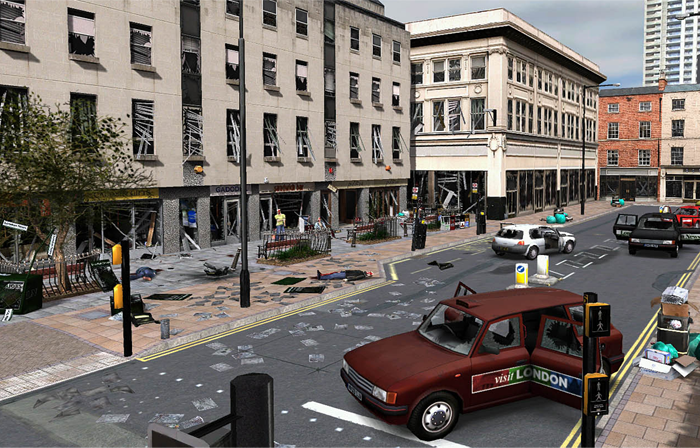
\includegraphics[scale=0.5]{tics/images/triage.png}
\caption{Ambientación de Triage}
\label{fig:triage}
\end{figure}

\emph{Triage Trainer} está diseñado para formar profesionales (médicos, enfermeros, 
paramédicos, rescatistas) que puedan participar en una escena de un incidente 
mayor, en este caso el escenario se presenta como una explosión en una calle 
(ver figura~\ref{fig:triage}). Los jugadores deben realizar un triage, es decir, evaluar 
el grado de las lesiones de las víctimas, las cuales son generadas aleatoriamente, 
utilizando los protocolos y controles médicos adecuados, además de priorizar a las 
víctimas para el tratamiento. La apariencia física de cada víctima es imitada con 
precisión como los signos vitales, los síntomas y sobre todo los patrones de tiempo 
para el deterioro de las lesiones, es decir, la condición de una víctima cambia de 
forma realista con el tiempo (ver figura~\ref{fig:triage_patient1}).

\begin{figure}[ht!]
\centering 
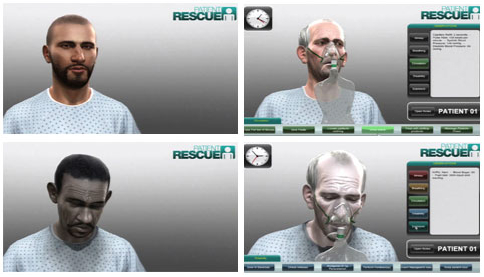
\includegraphics[scale=0.5]{tics/images/patient_side.jpg}
\caption{Evolución de un paciente en Triage}
\label{fig:triage_patient1}
\end{figure}

Al finalizar cada simulación los jugadores reciben retroalimentación acerca de
su rendimiento, incluyendo la precisión de sus chequeos, si los pacientes fueron
priorizados en el orden correcto y el tiempo que les llevó completar el triage,
en comparación con la de un experto.

La retroalimentación de los participantes que utilizaron \emph{Triage Trainer}
sugiere que el mismo cumplió exitosamente sus fines. Los jugadores asociaron su
experiencia en el videojuego con su experiencia en el mundo real y muchos de
ellos sentían que realmente estaban allí. Se espera que los jugadores puedan
tomar decisiones bajo presión, lo que ayudará a su desarrollo cognitivo. También
se observó que los jugadores tienden a discutir sus experiencias con sus
compañeros de curso, lo que también podría tener un impacto en su aprendizaje.

Un elemento que no fue evaluado por \emph{TruSim} debido a que no es
logísticamente posible es el impacto de las pruebas en la retención del
conocimiento y el cambio de comportamiento de los
jugadores\cite{education:games}. 


\subsection{SimVenture}

\begin{itemize}
\item \textbf{Tipo:} Juego de simulación de negocios.
\item \textbf{Destinatarios:} Personas de 14 a 30 años.
\item \textbf{Contenido:} Las realidades de la creación y funcionamiento de un
    negocio.
\item \textbf{Desarrollador:} \emph{Venture Simulations.}
\end{itemize}

En el inicio del videojuego (ver figura~\ref{fig:simventure_tutorial}), a los jugadores se
les brinda informaciones y antecedentes para que que se ubiquen en escena. Ellos
deben empezar a dirigir su propio negocio de fabricación y venta de
computadoras en sus casa, mientras deben mantener un trabajo de tiempo completo
independiente. El videojuego lleva a los jugadores a la ejecución de un negocio en su
propia casa y a la extensión del mismo a más locales, lo que requiere
contratación de personal. Los jugadores son capaces de avanzar en el videojuego a
través del aprendizaje de los elementos importantes de la empresa, organizadas
en cuatro categorías: organización, ventas/marketing, finanzas y operaciones.
Los jugadores toman decisiones acerca de las actividades dentro de estas áreas y
observan los resultados de sus acciones. 

\begin{figure}[ht!]
\centering 
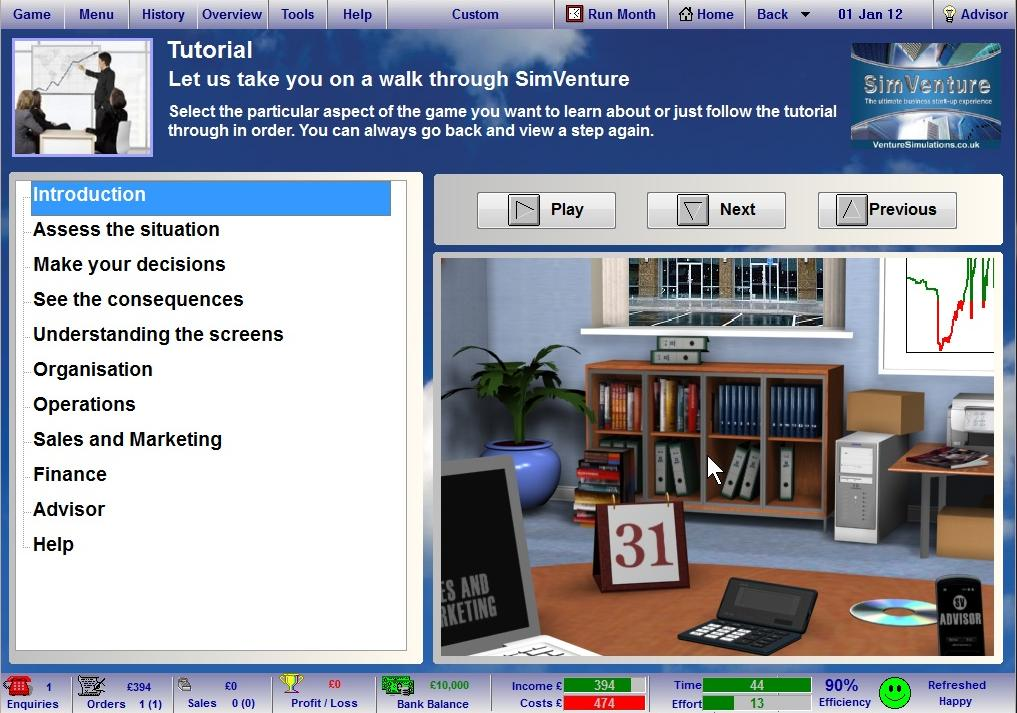
\includegraphics[scale=0.5]{tics/images/simventure-tutorial.jpg}
\caption{Tutorial de SimVenture}
\label{fig:simventure_tutorial}
\end{figure}

Los jugadores obtienen retroalimentación sobre un número de diferentes
parámetros. En un nivel básico, se puede simplemente revisar la cantidad de
ingresos que están generando. Además de esto, el éxito puede ser medido por la
cantidad de pedidos que han recibido para sus productos. También se proporciona
retroalimentación visual para representar la eficiencia de la organización y su
felicidad como individuo.

\emph{Phil Warren}, director de estudios de negocios en \emph{Snaith School}, ha
utilizado \emph{SimVenture} como complemento al plan de estudios. Según el
mismo, el plan de estudios por lo general sólo requiere que los estudiantes
aprendan sobre los diversos elementos del negocio de forma aislada, sin embargo
en la realidad, cualquier decisión que se tome en una de las partes de un
negocio tiene efecto en las demás. \emph{SimVenture} se vio como una oportunidad
de aplicar los conocimientos aprendidos en clase en una actividad práctica,
además se observó que permitir que los estudiantes jueguen en pares da un
espacio para la discusión en torno a las decisiones y aprenden de sus errores
juntos\cite{education:games}.

\section{Actualidad}

La relación de los videojuegos con el aprendizaje surge en los años $80$ y ha
llegado hasta la actualidad en plena efervescencia, siendo aplicados en varios
ámbitos de la educación tanto formal como no formal. Los juegos serios para el
entrenamiento de habilidades se pueden considerar una evolución de las técnicas
de entrenamiento basadas en la realidad virtual que se desarrollaron en los años
$90$ y que en la actualidad se han transformado, por su potencial motivacional,
de simulaciones puras a juegos\cite{videojuegos:gonzaleztardon}.

Al ser un área de creciente interés, existe una gran cantidad de conferencias
cuyo objetivo es el estudio de los juegos serios en la educación, a continuación
se presenta un resumen de algunas de ellas:

\begin{itemize}
\item \textbf{Games beyond Entertainment Week}: es una serie de conferencias
    cuyo objetivo es explorar los juegos serios, sus oportunidades de mercado,
    se centra en redes, promoción, desarrollo comercial. Una de sus
    conferencias, es la \emph{Games for health}, la cual se enfoca
    específicamente en el cuidado de la salud, agrupa a profesionales de la
    salud y de los juegos serios\cite{games_beyond_entertainment}.
\item \textbf{Serious games Development and Applications}: es una conferencia
    que se desarrolla desde el $2010$, apunta a coleccionar y distribuir todo el
    conocimiento relacionado a los juegos serios, para así proveer un foro de
    discusión sobre la actualidad del desarrollo de los juegos
    serios\cite{sgda}.
\item \textbf{Gaming and Learning Conference}: es una conferencia dedicada al
    estudio y aplicación de los juegos serios, incluye una presentación donde
    los desarrolladores pueden mostrar sus productos. Se interesa además en
    potenciales inversores para el desarrollo de videojuegos, así como en 
    desarrolladores, investigadores y jugadores\cite{gala}.
\item \textbf{Serious Play Conference}: es una conferencia dedicada a expertos
    con poder de decisión sobre organizaciones gubernamentales, el foco
    principal de la conferencia es explorar las oportunidades, desafíos y
    potencial de juegos serios desarrollados por los
    participantes\cite{seriousplay}.
\end{itemize}

Existen otras conferencias que no se centran exclusivamente en los juegos
serios, pero que por su naturaleza incluyen presentaciones sobre el tema, por
ejemplo, la \emph{DiGRA} (\textit{Digital Games Research Association}), se
centra en el desarrollo y la investigación de los videojuegos en general, pero
se han presentado numerosos artículos relacionados a  los juegos serios; la
\emph{Vs-Games}, que trata sobre entornos virtuales y videojuegos con
aplicaciones más allá del entretenimiento. Estas conferencias abarcan diferentes
áreas o ámbitos de aplicación de los juegos serios, que van desde lo militar
hasta el cuidado de la salud.


